\chapter{State of the Art} \label{chap:sota}
% TODO: pick a new name for this chapter, according to the domain

\section{Background} \label{sec:background}

\section{Related Work} \label{sec:related}

\section{Existing Technologies} \label{sec:existing}

\subsection{WaveNet} \label{subsec:tech-wavenet}
% TODO
\cite{oord_wavenet_2016}

A single WaveNet can capture the characteristics of many different speakers with equal fidelity, and can switch between them by conditioning on the speaker identity. When trained to model music, we find that it generates novel and often highly realistic musical fragments.

The dataset consisted of 44 hours of data from 109 different speakers.

Because the model is not conditioned on text, it generates non-existent but human language-like words in a smooth way with realistic sounding intonations. This is similar to generative models of language or images, where samples look realistic at first glance, but are clearly unnatural upon closer inspection. The lack of long range coherence is partly due to the limited size of the model's receptive field (about 300 milliseconds), which means it can only remember the last 2-3 phonemes it produced.

Finally, we observed that the model also picked up on other characteristics in the audio apart from the voice itself. For instance, it also mimicked the acoustics and recording quality, as well as the breathing and mouth movements of the speakers.

Even with a receptive field of several seconds, the models did not enforce long-range consistency which resulted in second-to-second variations in genre, instrumentation, volume and sound quality. Nevertheless, the samples were often harmonic and aesthetically pleasing, even when produced by unconditional models.

When applied to TTS, WaveNets produced samples that outperform the current best TTS systems in subjective naturalness. Finally, WaveNets showed very promising results when applied to music audio modeling and speech recognition.

Previously, autoregressive models like WaveNet (used in NSynth) represented the state of the art in neural audio synthesis. These models are good at learning the characteristics of sounds over very short time periods (local latent structure) but struggle with longerterm features (global latent structure). They are also very slow, since they have to generate waveforms one sample at a time. In contrast, GANs are capable of modeling global latent structure, as well as synthesising more efficiently. \cite{tahiroglu_-terity_2020}

\section{Approaches to Related Problems} \label{sec:approaches}

\subsection{WaveNet} \label{subsec:approach-wavenet}

% TODO
By using causal convolutions, we make sure the model cannot violate the ordering in which we model the data: the prediction p (xt+1 | x1, ..., xt) emitted by the model at timestep t cannot depend on any of the future timesteps xt+1, xt+2, . . . , xT as shown in Fig. \ref{fig:causal-convolution}. \cite{oord_wavenet_2016}

\begin{figure}[h]
    \caption{Causal convolution.}
    \centering
    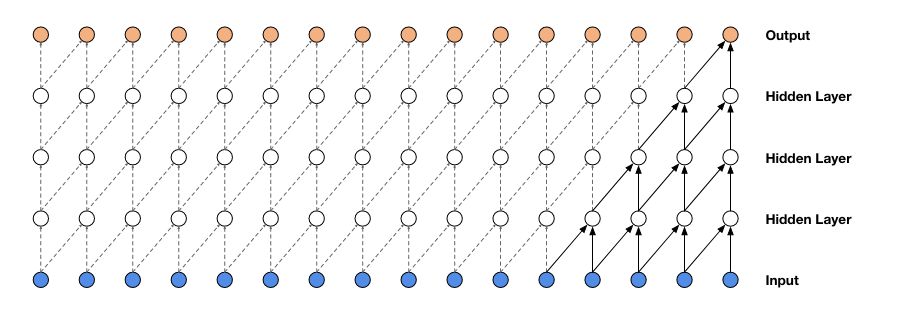
\includegraphics[width=\textwidth]{causal-convolution}
    \label{fig:causal-convolution}
\end{figure}

One of the problems of causal convolutions is that they require many layers, or large filters to increase the receptive field.

A dilated convolution (also called ` a trous, or convolution with holes) is a convolution where the filter is applied over an area larger than its length by skipping input values with a certain step. Fig. \ref{fig:dilated-convolution} shows a dilated convolution.

\begin{figure}[h]
    \caption{Dilated convolution.}
    \centering
    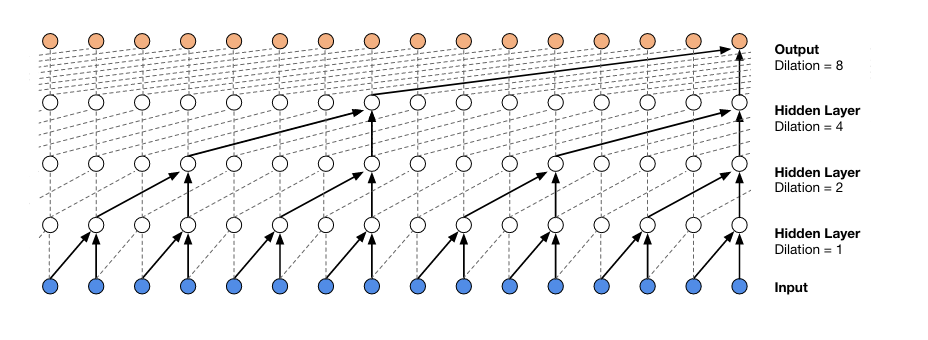
\includegraphics[width=\textwidth]{dilated-convolution}
    \label{fig:dilated-convolution}
\end{figure}

Stacked dilated convolutions enable networks to have very large receptive fields with just a few layers, while preserving the input resolution throughout the network as well as computational efficiency.

By conditioning the model on other input variables, we can guide WaveNet's generation to produce audio with the required characteristics. For example, in a multi-speaker setting we can choose the speaker by feeding the speaker identity to the model as an extra input. Similarly, for TTS we need to feed information about the text as an extra input.

if a model is not conditioned on text, it will generate human-like sounds without any meaning behind it

these models also capture extra sounds such as the breathing and background noises